%\VignetteDepends{knitr}
%\VignetteIndexEntry{An introduction to GAGA}
%\VignetteCompiler{knitr}
%\VignetteEngine{knitr::knitr}

\documentclass{article}

% LaTeX packages 
\usepackage{hyperref} % For hyperlinks\
\usepackage{float} % for floating images
\usepackage{alltt} % for verbatim blocks of text

% This block sets all links to be black and removes the hideous coloured boxes around them
\hypersetup{
    colorlinks=true,
    linkcolor=black,
    citecolor=black,
    filecolor=black,
    urlcolor=black,
}

\usepackage{Sweave}
\begin{document}
\Sconcordance{concordance:GAGA_vignette.tex:GAGA_vignette.Rnw:%
1 11 1 1 0 14 1 1 3 2 0 1 1 1 2 4 0 1 2 20 1 1 3 2 0 1 3 1 0 1 4 12 0 1 %
2 1 3 5 0 1 2 3 1 13 0 1 12 12 1}


\title{An introduction to GAGA}
\author{Alex Murison and Christopher P Wardell, alex.murison@icr.ac.uk}
\maketitle

This vignette serves as an introduction to the R package GAGA.  It covers the basic use cases and usage of the package, explaining the input and output and contains several worked examples.  If you use this package, please cite: (CITATION).

\paragraph{Installation:} The latest stable version can be installed from Bioconductor here...
 
\begin{Schunk}
\begin{Sinput}
> ## Install
> source("http://bioconductor.org/biocLite.R")
> biocLite("GAGA")
> ## Load
> library(GAGA)
\end{Sinput}
\end{Schunk}

The latest development version can be cloned from our GitHub here: \href{https://github.com/MurisonWardell}{https://github.com/MurisonWardell} but must be built from source.

\pagebreak
\tableofcontents
\pagebreak

\section{Overview}
\subsection{Introduction}
We work extensively with sequencing data, particularly next-generation sequencing data from tumour-normal pairs.  The tumour genome contains many single nucleotide variants (SNVs) which are single-base differences between the tumour sample and the reference genome.  These can be separated into two groups:

\begin{enumerate}
   \item SNVs shared between tumour and normal samples.  These are germline variants and were present before the tumour
   \item SNVs only present in the tumour sample.  These are somatic mutations
\end{enumerate}

Tumours are known to be heterogeneous populations of related cells and in any given tumour sample there may be differing proportions of cells that contain certain SNVs.  These proportions can be calculated for each SNV in turn using the number of supporting reads, the read depth and the copy number of that region.  These proportions are termed the cancer cell fraction (CCF) and range between 0 (no cells contain the SNV in that sample) to 1 (all cells contain the SNV in that sample).

The SNV CCF values can be explained as a mixture of a number of related clones.  We know that SNVs are heritable characteristics between clones and that new clones arise and go extinct over time.


\subsection{Genetic algorithms}
Overview of genetic algorithms and the string encoding each individual.
\subsection{GAGA input}
\subsection{GAGA output}

Discussion that you might get a different answer every time and that the number of clones is probably the most important variable.  The user MUST cycle through a number of clones and choose the lowest number of clones with the best answer.  INCLUDE SAMPLE CODE!


\section{Worked examples}
A number of sample data sets are distributed with the GAGA package and are discussed in order of increasing complexity.
\subsection{Example 1 - simple synthetic data}
A very small and simple synthetic data set is included.  To demonstrate that your GAGA installation is working, you can execute the following commands.  
\begin{Schunk}
\begin{Sinput}
> ## Load library
> library(GAGA)
> ## Load simple data set
> data("gaga_simple_data")
> ## There  are three columns (time points T0, T1 and T2)
> ## and three rows (mutations M1, M2, M3)
> gaga_simple_data
\end{Sinput}
\begin{Soutput}
  names T0  T1  T2
1    M1  1 1.0 1.0
2    M2  0 0.7 1.0
3    M3  0 0.0 0.8
\end{Soutput}
\end{Schunk}

As we know the true number and relationship between the clones, we specify these and run the algorithm.  It should converge at the minimum score of zero quite quickly and exit after 200 generations of coverging at the highest fitness value.

\begin{Schunk}
\begin{Sinput}
> ## Execute gaga() function on the simple data set
> simpleDataSolution=gaga(gaga_simple_data, number_of_clones=3, nroot=1,iterations=1000)
\end{Sinput}
\end{Schunk}

We can view the highest scoring solution(s) by accessing the appropriate slot in the returned object.  For example:

\begin{Schunk}
\begin{Sinput}
> ## Access solution slot in returned object to show highest scoring solution(s)
> simpleDataSolution@solution
\end{Sinput}
\end{Schunk}
% Note; this R code snippet isn't in a regular knitr code block on purpose to make it appear as if it has been run
\begin{alltt}
     x1 x2 x3 x4 x5 x6 x7 x8 x9 x10 x11 x12 x13 x14 x15
[1,]  0  1  2  5  0  0  3  7  0   0   1   4   1   2   3
[2,]  0  1  2  7  0  0  3  7  0   0   1   4   1   2   3
[3,]  0  1  2  1  0  0  3  7  0   0   1   4   1   2   3
[4,]  0  1  2  6  0  0  3  7  0   0   1   4   1   2   3
[5,]  0  1  2  3  0  0  3  7  0   0   1   4   1   2   3
[6,]  0  1  2 11  0  0  3  7  0   0   1   4   1   2   3
[7,]  0  1  2 12  0  0  3  7  0   0   1   4   1   2   3
\end{alltt}

Note that it's possible for multiple solutions to have equally good fitness scores which may encode different phylogenies, mutation distributions or proportions.  However, in this case all of the solutions are numerically identical and exist because of the degeneracy in the way that the clonal proportions are encoded.

We can now examine the best solution(s) using the gagaReport() function.  

\begin{Schunk}
\begin{Sinput}
> ## Produce plots for the phylogeny, heatmap and proportions in turn
> gagaReport(gaga_simple_data,simpleDataSolution,outType="phylogeny")
> gagaReport(gaga_simple_data,simpleDataSolution,outType="heatmap")
> gagaReport(gaga_simple_data,simpleDataSolution,outType="proportion")
> ## Create output files representing the solution(s) in the current working directory
> gagaReport(gaga_simple_data,simpleDataSolution,outType="complete")
> ## In case you want to know the current working directory, it can be reported using this function:
> getwd()
\end{Sinput}
\end{Schunk}

You should see images like those below.  The colours used for clones are consistent between the phylogeny, the sidebar of the heatmap and the proportion barplot.

\begin{figure}[H]
    \centering
    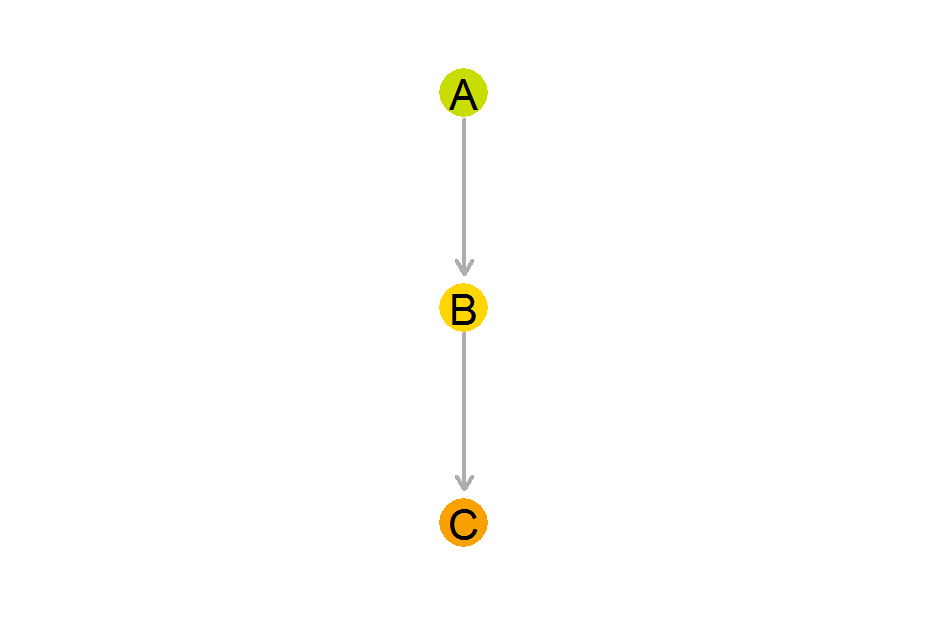
\includegraphics{gaga_simple_data_phylogeny.png}
    \caption{The phylogeny of the optimum solution to the simple data set.  There is a single root (clone A) which gives rise to clone B which gives rise to clone C.}
\end{figure}

\begin{figure}[H]
   \centering
       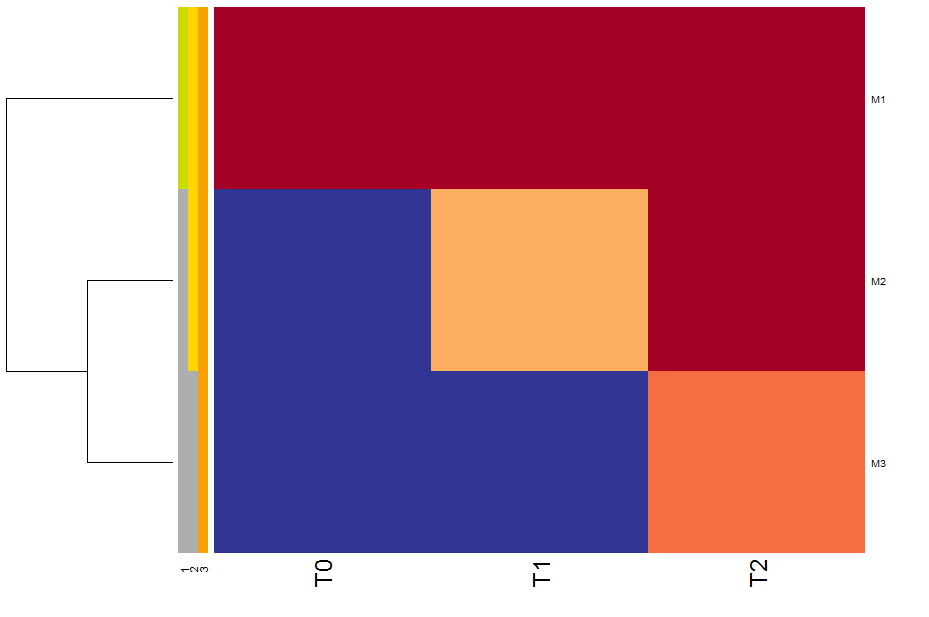
\includegraphics{gaga_simple_data_heatmap}
   \caption{The input data has been clustered using the heatmap.plus package.  The colour scale goes from blue (low values) through yellow to red (high values).
   The coloured sidebar shows which clones contain which mutations.  For example, M1 is contained by all clones, whereas M3 is contained only by clone C.}
\end{figure}

\begin{figure}[H]
   \centering
       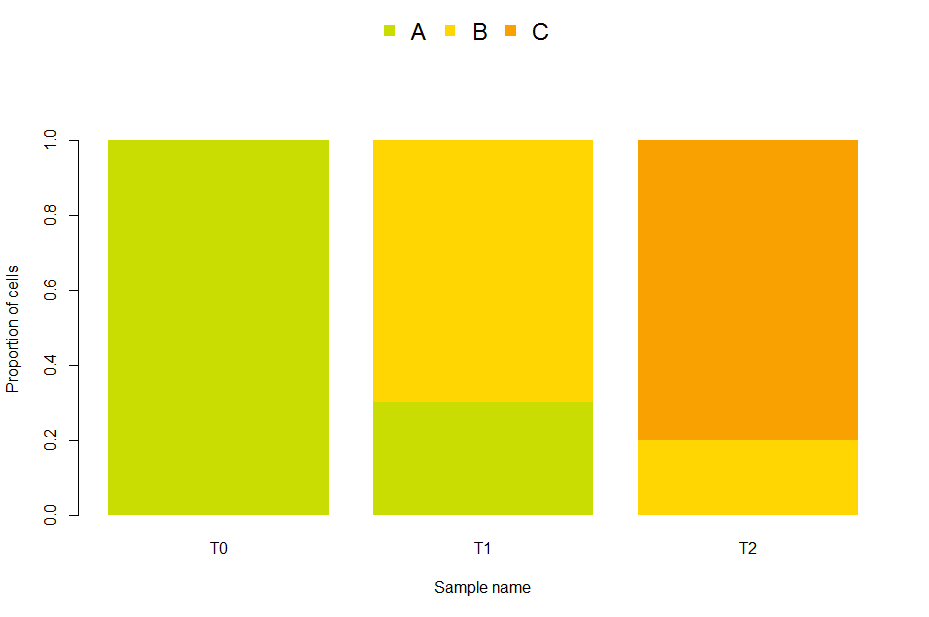
\includegraphics{gaga_simple_data_proportions}
   \caption{The proportions of each clone in each sample of the simple data set.  Sample T0 is composed entirely of clone A, whereas sample T1 is an unequal mixture of 
   clones A and B, while sample T2 is an unequal mixture of clones B and C.}
\end{figure}

\subsection{Example 2 - synthetic data containing a hidden clone}
The second synthetic data set demonstrates the ability of GAGA to infer intermediate clones that are not explicitly detected in the input data and therefore "hidden".

\begin{Schunk}
\begin{Sinput}
> ## Load library
> library(GAGA)
> ## Load hidden data set
> data("gaga_hidden_data")
> ## There  are three columns (time points T0, T1 and T2)
> ## and five rows (mutations M1, M2, M3, M4 and M5)
> gaga_hidden_data
\end{Sinput}
\begin{Soutput}
  names T0  T1  T2
1    M1  1 1.0 1.0
2    M2  0 0.5 1.0
3    M3  0 0.3 0.7
4    M4  0 0.2 0.3
5    M5  0 0.0 0.6
\end{Soutput}
\end{Schunk}

\begin{Schunk}
\begin{Sinput}
> ## Execute gaga() function on the hidden data set
> hiddenDataSolution=gaga(gaga_hidden_data, number_of_clones=5, nroot=1,iterations=3000)
> ## Access solution slot in returned object to show highest scoring solution(s)
> ## This solution's score is -0.02500000
> hiddenDataSolution@solution
\end{Sinput}
\end{Schunk}
% Note; this R code snippet isn't in a regular knitr code block on purpose to make it appear as if it has been run
\begin{alltt}
     x1 x2 x3 x4 x5 x6 x7 x8 x9 x10 x11 x12 x13 x14 x15 x16 x17 x18 x19 x20 x21 x22 x23 x24 x25
[1,]  0  1  2  2  4 29  0  0  0   0   8   0   3   5   0   0   0   6   2  12   1   2   4   3   5
\end{alltt}

\begin{Schunk}
\begin{Sinput}
> ## Produce plots for the phylogeny, heatmap and proportions in turn
> gagaReport(gaga_hidden_data,hiddenDataSolution,outType="phylogeny")
> gagaReport(gaga_hidden_data,hiddenDataSolution,outType="heatmap")
> gagaReport(gaga_hidden_data,hiddenDataSolution,outType="proportion")
> ## Create output files representing the solution(s) in the current working directory
> gagaReport(gaga_simple_data,simpleDataSolution,outType="complete")
\end{Sinput}
\end{Schunk}

\begin{figure}[H]
    \centering
    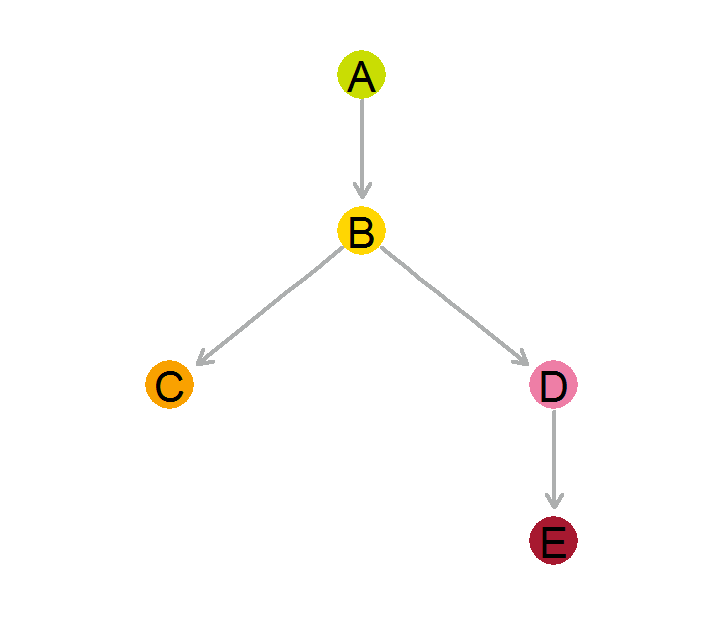
\includegraphics{gaga_hidden_data_phylogeny.png}
    \caption{The phylogeny of the optimum solution to the hidden data set.  Clone B is both the child of clone A and the parent of all other clones.}
\end{figure}

\begin{figure}[H]
   \centering
       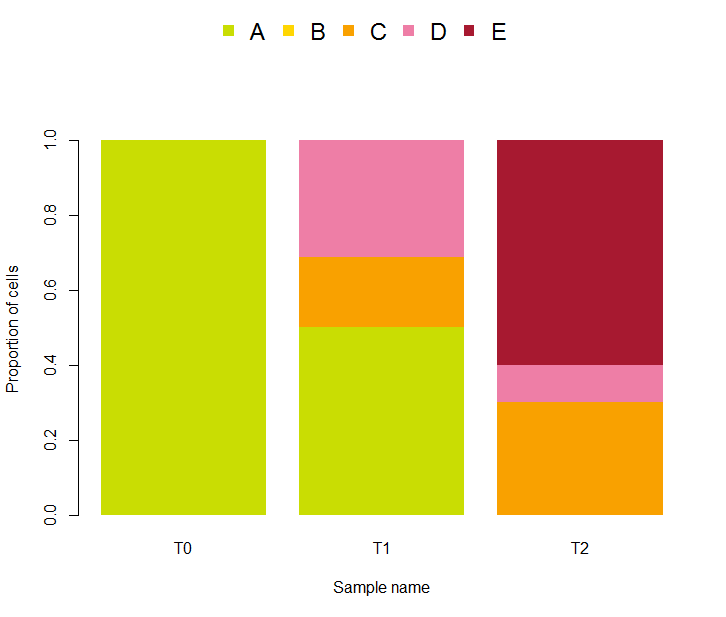
\includegraphics{gaga_hidden_data_proportions}
   \caption{The proportions of each clone in each sample of the hidden data set.  Although clone B is not present in any of the samples its existance and ancestry have been correctly inferred.}
\end{figure}

\subsection{Example 3 - complex synthetic data and noisy data}
These synthetic data are close to the sort of observations produced by a typical tumour-normal paired exome sequencing experiment.  There are four time points (T0 to T3) and 90 mutations (gene1 to gene90).  Each of the values represents the proportion of cells that contain that mutation at that time point - the cancer cell fraction (CCF).




JITTERED DATA

\subsection{Example 4}
The yeast data, as it's REAL data and has a (relatively) definite answer AND is contaminated.
\subsection{Example 5}
Perhaps include the data from the recent LM paper?
\subsection{Advanced GAGA usage and best practices}
Demonstrate proper usage; how to iterate over many clones and estimate how many clones there are, then performing many runs




\end{document}
